\documentclass[1p]{elsarticle_modified}
%\bibliographystyle{elsarticle-num}

%\usepackage[colorlinks]{hyperref}
%\usepackage{abbrmath_seonhwa} %\Abb, \Ascr, \Acal ,\Abf, \Afrak
\usepackage{amsfonts}
\usepackage{amssymb}
\usepackage{amsmath}
\usepackage{amsthm}
\usepackage{scalefnt}
\usepackage{amsbsy}
\usepackage{kotex}
\usepackage{caption}
\usepackage{subfig}
\usepackage{color}
\usepackage{graphicx}
\usepackage{xcolor} %% white, black, red, green, blue, cyan, magenta, yellow
\usepackage{float}
\usepackage{setspace}
\usepackage{hyperref}

\usepackage{tikz}
\usetikzlibrary{arrows}

\usepackage{multirow}
\usepackage{array} % fixed length table
\usepackage{hhline}

%%%%%%%%%%%%%%%%%%%%%
\makeatletter
\renewcommand*\env@matrix[1][\arraystretch]{%
	\edef\arraystretch{#1}%
	\hskip -\arraycolsep
	\let\@ifnextchar\new@ifnextchar
	\array{*\c@MaxMatrixCols c}}
\makeatother %https://tex.stackexchange.com/questions/14071/how-can-i-increase-the-line-spacing-in-a-matrix
%%%%%%%%%%%%%%%

\usepackage[normalem]{ulem}

\newcommand{\msout}[1]{\ifmmode\text{\sout{\ensuremath{#1}}}\else\sout{#1}\fi}
%SOURCE: \msout is \stkout macro in https://tex.stackexchange.com/questions/20609/strikeout-in-math-mode

\newcommand{\cancel}[1]{
	\ifmmode
	{\color{red}\msout{#1}}
	\else
	{\color{red}\sout{#1}}
	\fi
}

\newcommand{\add}[1]{
	{\color{blue}\uwave{#1}}
}

\newcommand{\replace}[2]{
	\ifmmode
	{\color{red}\msout{#1}}{\color{blue}\uwave{#2}}
	\else
	{\color{red}\sout{#1}}{\color{blue}\uwave{#2}}
	\fi
}

\newcommand{\Sol}{\mathcal{S}} %segment
\newcommand{\D}{D} %diagram
\newcommand{\A}{\mathcal{A}} %arc


%%%%%%%%%%%%%%%%%%%%%%%%%%%%%5 test

\def\sl{\operatorname{\textup{SL}}(2,\Cbb)}
\def\psl{\operatorname{\textup{PSL}}(2,\Cbb)}
\def\quan{\mkern 1mu \triangleright \mkern 1mu}

\theoremstyle{definition}
\newtheorem{thm}{Theorem}[section]
\newtheorem{prop}[thm]{Proposition}
\newtheorem{lem}[thm]{Lemma}
\newtheorem{ques}[thm]{Question}
\newtheorem{cor}[thm]{Corollary}
\newtheorem{defn}[thm]{Definition}
\newtheorem{exam}[thm]{Example}
\newtheorem{rmk}[thm]{Remark}
\newtheorem{alg}[thm]{Algorithm}

\newcommand{\I}{\sqrt{-1}}
\begin{document}

%\begin{frontmatter}
%
%\title{Boundary parabolic representations of knots up to 8 crossings}
%
%%% Group authors per affiliation:
%\author{Yunhi Cho} 
%\address{Department of Mathematics, University of Seoul, Seoul, Korea}
%\ead{yhcho@uos.ac.kr}
%
%
%\author{Seonhwa Kim} %\fnref{s_kim}}
%\address{Center for Geometry and Physics, Institute for Basic Science, Pohang, 37673, Korea}
%\ead{ryeona17@ibs.re.kr}
%
%\author{Hyuk Kim}
%\address{Department of Mathematical Sciences, Seoul National University, Seoul 08826, Korea}
%\ead{hyukkim@snu.ac.kr}
%
%\author{Seokbeom Yoon}
%\address{Department of Mathematical Sciences, Seoul National University, Seoul, 08826,  Korea}
%\ead{sbyoon15@snu.ac.kr}
%
%\begin{abstract}
%We find all boundary parabolic representation of knots up to 8 crossings.
%
%\end{abstract}
%\begin{keyword}
%    \MSC[2010] 57M25 
%\end{keyword}
%
%\end{frontmatter}

%\linenumbers
%\tableofcontents
%
\newcommand\colored[1]{\textcolor{white}{\rule[-0.35ex]{0.8em}{1.4ex}}\kern-0.8em\color{red} #1}%
%\newcommand\colored[1]{\textcolor{white}{ #1}\kern-2.17ex	\textcolor{white}{ #1}\kern-1.81ex	\textcolor{white}{ #1}\kern-2.15ex\color{red}#1	}

{\Large $\underline{11n_{159}~(K11n_{159})}$}

\setlength{\tabcolsep}{10pt}
\renewcommand{\arraystretch}{1.6}
\vspace{1cm}\begin{tabular}{m{100pt}>{\centering\arraybackslash}m{274pt}}
\multirow{5}{120pt}{
	\centering
	\includegraphics[width=112pt]{../../../GIT/diagram.site/Diagrams/png/775_11n_159.png}\\
\ \ \ A knot diagram\footnotemark}&
\allowdisplaybreaks
\textbf{Linearized knot diagam} \\
\cline{2-2}
 &
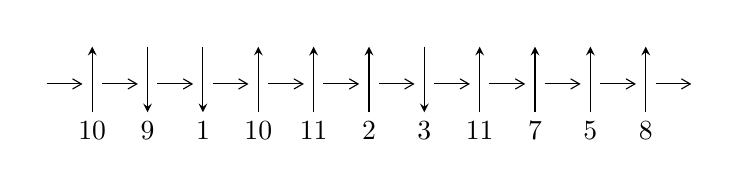
\begin{tikzpicture}[x=20pt, y=17pt]
	% nodes
	\node (C0) at (0, 0) {};
	\node (C1) at (1, 0) {};
	\node (C1U) at (1, +1) {};
	\node (C1D) at (1, -1) {10};

	\node (C2) at (2, 0) {};
	\node (C2U) at (2, +1) {};
	\node (C2D) at (2, -1) {9};

	\node (C3) at (3, 0) {};
	\node (C3U) at (3, +1) {};
	\node (C3D) at (3, -1) {1};

	\node (C4) at (4, 0) {};
	\node (C4U) at (4, +1) {};
	\node (C4D) at (4, -1) {10};

	\node (C5) at (5, 0) {};
	\node (C5U) at (5, +1) {};
	\node (C5D) at (5, -1) {11};

	\node (C6) at (6, 0) {};
	\node (C6U) at (6, +1) {};
	\node (C6D) at (6, -1) {2};

	\node (C7) at (7, 0) {};
	\node (C7U) at (7, +1) {};
	\node (C7D) at (7, -1) {3};

	\node (C8) at (8, 0) {};
	\node (C8U) at (8, +1) {};
	\node (C8D) at (8, -1) {11};

	\node (C9) at (9, 0) {};
	\node (C9U) at (9, +1) {};
	\node (C9D) at (9, -1) {7};

	\node (C10) at (10, 0) {};
	\node (C10U) at (10, +1) {};
	\node (C10D) at (10, -1) {5};

	\node (C11) at (11, 0) {};
	\node (C11U) at (11, +1) {};
	\node (C11D) at (11, -1) {8};
	\node (C12) at (12, 0) {};

	% arrows
	\draw[->,>={angle 60}]
	(C0) edge (C1) (C1) edge (C2) (C2) edge (C3) (C3) edge (C4) (C4) edge (C5) (C5) edge (C6) (C6) edge (C7) (C7) edge (C8) (C8) edge (C9) (C9) edge (C10) (C10) edge (C11) (C11) edge (C12) ;	\draw[->,>=stealth]
	(C1D) edge (C1U) (C2U) edge (C2D) (C3U) edge (C3D) (C4D) edge (C4U) (C5D) edge (C5U) (C6D) edge (C6U) (C7U) edge (C7D) (C8D) edge (C8U) (C9D) edge (C9U) (C10D) edge (C10U) (C11D) edge (C11U) ;
	\end{tikzpicture} \\
\hhline{~~} \\& 
\textbf{Solving Sequence} \\ \cline{2-2} 
 &
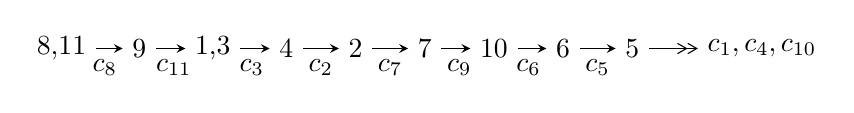
\begin{tikzpicture}[x=25pt, y=7pt]
	% node
	\node (A0) at (-1/8, 0) {8,11};
	\node (A1) at (1, 0) {9};
	\node (A2) at (33/16, 0) {1,3};
	\node (A3) at (25/8, 0) {4};
	\node (A4) at (33/8, 0) {2};
	\node (A5) at (41/8, 0) {7};
	\node (A6) at (49/8, 0) {10};
	\node (A7) at (57/8, 0) {6};
	\node (A8) at (65/8, 0) {5};
	\node (C1) at (1/2, -1) {$c_{8}$};
	\node (C2) at (3/2, -1) {$c_{11}$};
	\node (C3) at (21/8, -1) {$c_{3}$};
	\node (C4) at (29/8, -1) {$c_{2}$};
	\node (C5) at (37/8, -1) {$c_{7}$};
	\node (C6) at (45/8, -1) {$c_{9}$};
	\node (C7) at (53/8, -1) {$c_{6}$};
	\node (C8) at (61/8, -1) {$c_{5}$};
	\node (A9) at (10, 0) {$c_{1},c_{4},c_{10}$};

	% edge
	\draw[->,>=stealth]	
	(A0) edge (A1) (A1) edge (A2) (A2) edge (A3) (A3) edge (A4) (A4) edge (A5) (A5) edge (A6) (A6) edge (A7) (A7) edge (A8) ;
	\draw[->>,>={angle 60}]	
	(A8) edge (A9);
\end{tikzpicture} \\ 

\end{tabular} \\

\footnotetext{
The image of knot diagram is generated by the software ``\textbf{Draw programme}" developed by Andrew Bartholomew(\url{http://www.layer8.co.uk/maths/draw/index.htm\#Running-draw}), where we modified some parts for our purpose(\url{https://github.com/CATsTAILs/LinksPainter}).
}\phantom \\ \newline 
\centering \textbf{Ideals for irreducible components\footnotemark of $X_{\text{par}}$} 
 
\begin{align*}
I^u_{1}&=\langle 
4.18672\times10^{96} u^{50}-1.99216\times10^{96} u^{49}+\cdots+1.57066\times10^{97} b-7.53117\times10^{96},\\
\phantom{I^u_{1}}&\phantom{= \langle  }6.93809\times10^{95} u^{50}-3.65626\times10^{96} u^{49}+\cdots+1.57066\times10^{97} a-2.77787\times10^{98},\;u^{51}+19 u^{49}+\cdots+13 u+1\rangle \\
I^u_{2}&=\langle 
- u^{15}- u^{14}-3 u^{13}- u^{12}+u^{11}+6 u^{10}+14 u^9+16 u^8+22 u^7+15 u^6+14 u^5+6 u^4+7 u^3+u^2+b,\\
\phantom{I^u_{2}}&\phantom{= \langle  }-201 u^{15}-115 u^{14}+\cdots+85 a-229,\;u^{16}+u^{15}+\cdots- u-1\rangle \\
\\
\end{align*}
\raggedright * 2 irreducible components of $\dim_{\mathbb{C}}=0$, with total 67 representations.\\
\footnotetext{All coefficients of polynomials are rational numbers. But the coefficients are sometimes approximated in decimal forms when there is not enough margin.}
\newpage
\renewcommand{\arraystretch}{1}
\centering \section*{I. $I^u_{1}= \langle 4.19\times10^{96} u^{50}-1.99\times10^{96} u^{49}+\cdots+1.57\times10^{97} b-7.53\times10^{96},\;6.94\times10^{95} u^{50}-3.66\times10^{96} u^{49}+\cdots+1.57\times10^{97} a-2.78\times10^{98},\;u^{51}+19 u^{49}+\cdots+13 u+1 \rangle$}
\flushleft \textbf{(i) Arc colorings}\\
\begin{tabular}{m{7pt} m{180pt} m{7pt} m{180pt} }
\flushright $a_{8}=$&$\begin{pmatrix}1\\0\end{pmatrix}$ \\
\flushright $a_{11}=$&$\begin{pmatrix}0\\u\end{pmatrix}$ \\
\flushright $a_{9}=$&$\begin{pmatrix}1\\- u^2\end{pmatrix}$ \\
\flushright $a_{1}=$&$\begin{pmatrix}u\\u\end{pmatrix}$ \\
\flushright $a_{3}=$&$\begin{pmatrix}-0.0441731 u^{50}+0.232785 u^{49}+\cdots+101.687 u+17.6860\\-0.266558 u^{50}+0.126836 u^{49}+\cdots-2.22590 u+0.479491\end{pmatrix}$ \\
\flushright $a_{4}=$&$\begin{pmatrix}0.00694886 u^{50}+0.245771 u^{49}+\cdots+100.087 u+17.5801\\-0.215436 u^{50}+0.139822 u^{49}+\cdots-3.82562 u+0.373542\end{pmatrix}$ \\
\flushright $a_{2}=$&$\begin{pmatrix}-0.315201 u^{50}+0.322634 u^{49}+\cdots+96.4791 u+17.9327\\-0.255159 u^{50}+0.144501 u^{49}+\cdots-1.32888 u+0.569340\end{pmatrix}$ \\
\flushright $a_{7}=$&$\begin{pmatrix}0.492967 u^{50}-0.795819 u^{49}+\cdots-148.859 u-17.2613\\-0.135931 u^{50}-0.160168 u^{49}+\cdots-20.5135 u-2.00969\end{pmatrix}$ \\
\flushright $a_{10}=$&$\begin{pmatrix}-2.73260 u^{50}+0.0713461 u^{49}+\cdots-195.275 u-13.1506\\-0.141930 u^{50}+0.0517872 u^{49}+\cdots-5.44851 u+0.0702398\end{pmatrix}$ \\
\flushright $a_{6}=$&$\begin{pmatrix}2.17298 u^{50}-0.00432810 u^{49}+\cdots+193.781 u+17.3396\\0.0132709 u^{50}+0.0275351 u^{49}+\cdots+3.99076 u+0.0293163\end{pmatrix}$ \\
\flushright $a_{5}=$&$\begin{pmatrix}2.17298 u^{50}-0.00432810 u^{49}+\cdots+193.781 u+17.3396\\-0.0193853 u^{50}+0.0282101 u^{49}+\cdots+1.87404 u+0.0336444\end{pmatrix}$\\ \flushright $a_{5}=$&$\begin{pmatrix}2.17298 u^{50}-0.00432810 u^{49}+\cdots+193.781 u+17.3396\\-0.0193853 u^{50}+0.0282101 u^{49}+\cdots+1.87404 u+0.0336444\end{pmatrix}$\\&\end{tabular}
\flushleft \textbf{(ii) Obstruction class $= -1$}\\~\\
\flushleft \textbf{(iii) Cusp Shapes $= -0.101424 u^{50}+0.0191393 u^{49}+\cdots-6.99335 u+1.74681$}\\~\\
\newpage\renewcommand{\arraystretch}{1}
\flushleft \textbf{(iv) u-Polynomials at the component}\newline \\
\begin{tabular}{m{50pt}|m{274pt}}
Crossings & \hspace{64pt}u-Polynomials at each crossing \\
\hline $$\begin{aligned}c_{1}\end{aligned}$$&$\begin{aligned}
&u^{51}+4 u^{50}+\cdots+10304 u+1139
\end{aligned}$\\
\hline $$\begin{aligned}c_{2}\end{aligned}$$&$\begin{aligned}
&u^{51}+u^{50}+\cdots+197 u+3
\end{aligned}$\\
\hline $$\begin{aligned}c_{3}\end{aligned}$$&$\begin{aligned}
&u^{51}+4 u^{50}+\cdots-668 u+28
\end{aligned}$\\
\hline $$\begin{aligned}c_{4},c_{5},c_{10}\end{aligned}$$&$\begin{aligned}
&u^{51}+u^{50}+\cdots-15 u-1
\end{aligned}$\\
\hline $$\begin{aligned}c_{6}\end{aligned}$$&$\begin{aligned}
&u^{51}+14 u^{49}+\cdots-3611 u+487
\end{aligned}$\\
\hline $$\begin{aligned}c_{7}\end{aligned}$$&$\begin{aligned}
&u^{51}- u^{50}+\cdots+2734 u-367
\end{aligned}$\\
\hline $$\begin{aligned}c_{8},c_{11}\end{aligned}$$&$\begin{aligned}
&u^{51}+19 u^{49}+\cdots+13 u+1
\end{aligned}$\\
\hline $$\begin{aligned}c_{9}\end{aligned}$$&$\begin{aligned}
&u^{51}+3 u^{50}+\cdots+17 u+1
\end{aligned}$\\
\hline
\end{tabular}\\~\\
\newpage\renewcommand{\arraystretch}{1}
\flushleft \textbf{(v) Riley Polynomials at the component}\newline \\
\begin{tabular}{m{50pt}|m{274pt}}
Crossings & \hspace{64pt}Riley Polynomials at each crossing \\
\hline $$\begin{aligned}c_{1}\end{aligned}$$&$\begin{aligned}
&y^{51}+48 y^{50}+\cdots+51493582 y-1297321
\end{aligned}$\\
\hline $$\begin{aligned}c_{2}\end{aligned}$$&$\begin{aligned}
&y^{51}-11 y^{50}+\cdots+48673 y-9
\end{aligned}$\\
\hline $$\begin{aligned}c_{3}\end{aligned}$$&$\begin{aligned}
&y^{51}-54 y^{50}+\cdots+361104 y-784
\end{aligned}$\\
\hline $$\begin{aligned}c_{4},c_{5},c_{10}\end{aligned}$$&$\begin{aligned}
&y^{51}-13 y^{50}+\cdots+69 y-1
\end{aligned}$\\
\hline $$\begin{aligned}c_{6}\end{aligned}$$&$\begin{aligned}
&y^{51}+28 y^{50}+\cdots-14382675 y-237169
\end{aligned}$\\
\hline $$\begin{aligned}c_{7}\end{aligned}$$&$\begin{aligned}
&y^{51}-13 y^{50}+\cdots+4303142 y-134689
\end{aligned}$\\
\hline $$\begin{aligned}c_{8},c_{11}\end{aligned}$$&$\begin{aligned}
&y^{51}+38 y^{50}+\cdots-63 y-1
\end{aligned}$\\
\hline $$\begin{aligned}c_{9}\end{aligned}$$&$\begin{aligned}
&y^{51}+3 y^{50}+\cdots+231 y-1
\end{aligned}$\\
\hline
\end{tabular}\\~\\
\newpage\flushleft \textbf{(vi) Complex Volumes and Cusp Shapes}
$$\begin{array}{c|c|c}  
\text{Solutions to }I^u_{1}& \I (\text{vol} + \sqrt{-1}CS) & \text{Cusp shape}\\
 \hline 
\begin{aligned}
u &= -0.493427 + 0.809787 I \\
a &= -0.77037 + 1.28680 I \\
b &= -1.158320 - 0.268559 I\end{aligned}
 & -3.18456 - 2.09749 I & \phantom{-}1.52387 + 2.56668 I \\ \hline\begin{aligned}
u &= -0.493427 - 0.809787 I \\
a &= -0.77037 - 1.28680 I \\
b &= -1.158320 + 0.268559 I\end{aligned}
 & -3.18456 + 2.09749 I & \phantom{-}1.52387 - 2.56668 I \\ \hline\begin{aligned}
u &= \phantom{-}0.440430 + 1.030910 I \\
a &= \phantom{-}1.20909 + 0.73700 I \\
b &= \phantom{-}0.648815 + 0.030734 I\end{aligned}
 & -1.47252 + 3.57882 I & \phantom{-}5.00000 - 4.02671 I \\ \hline\begin{aligned}
u &= \phantom{-}0.440430 - 1.030910 I \\
a &= \phantom{-}1.20909 - 0.73700 I \\
b &= \phantom{-}0.648815 - 0.030734 I\end{aligned}
 & -1.47252 - 3.57882 I & \phantom{-}5.00000 + 4.02671 I \\ \hline\begin{aligned}
u &= -0.479467 + 1.026910 I \\
a &= -2.05858 + 0.43573 I \\
b &= -0.759278 - 0.845778 I\end{aligned}
 & -1.69267 - 6.49416 I & \phantom{-}2.47045 + 12.27311 I \\ \hline\begin{aligned}
u &= -0.479467 - 1.026910 I \\
a &= -2.05858 - 0.43573 I \\
b &= -0.759278 + 0.845778 I\end{aligned}
 & -1.69267 + 6.49416 I & \phantom{-}2.47045 - 12.27311 I \\ \hline\begin{aligned}
u &= \phantom{-}0.743842 + 0.386843 I \\
a &= \phantom{-}0.297848 + 0.032171 I \\
b &= \phantom{-}0.446197 + 0.593035 I\end{aligned}
 & \phantom{-}1.328990 + 0.424799 I & \phantom{-}9.68382 - 3.33114 I \\ \hline\begin{aligned}
u &= \phantom{-}0.743842 - 0.386843 I \\
a &= \phantom{-}0.297848 - 0.032171 I \\
b &= \phantom{-}0.446197 - 0.593035 I\end{aligned}
 & \phantom{-}1.328990 - 0.424799 I & \phantom{-}9.68382 + 3.33114 I \\ \hline\begin{aligned}
u &= \phantom{-}0.095349 + 1.173960 I \\
a &= -1.19574 - 0.93729 I \\
b &= -0.696664 - 0.158856 I\end{aligned}
 & -0.53609 - 2.28831 I & \phantom{-}3.93640 + 2.00082 I \\ \hline\begin{aligned}
u &= \phantom{-}0.095349 - 1.173960 I \\
a &= -1.19574 + 0.93729 I \\
b &= -0.696664 + 0.158856 I\end{aligned}
 & -0.53609 + 2.28831 I & \phantom{-}3.93640 - 2.00082 I\\
 \hline 
 \end{array}$$\newpage$$\begin{array}{c|c|c}  
\text{Solutions to }I^u_{1}& \I (\text{vol} + \sqrt{-1}CS) & \text{Cusp shape}\\
 \hline 
\begin{aligned}
u &= \phantom{-}0.599757 + 1.068150 I \\
a &= \phantom{-}1.59872 + 0.52153 I \\
b &= \phantom{-}1.166950 - 0.515248 I\end{aligned}
 & -0.82395 + 4.71884 I & \phantom{-}8.89552 - 4.87376 I \\ \hline\begin{aligned}
u &= \phantom{-}0.599757 - 1.068150 I \\
a &= \phantom{-}1.59872 - 0.52153 I \\
b &= \phantom{-}1.166950 + 0.515248 I\end{aligned}
 & -0.82395 - 4.71884 I & \phantom{-}8.89552 + 4.87376 I \\ \hline\begin{aligned}
u &= -0.037987 + 0.741711 I \\
a &= \phantom{-}0.487424 - 0.496015 I \\
b &= -0.263663 + 1.061380 I\end{aligned}
 & \phantom{-}0.97092 + 2.65596 I & -1.16196 - 5.22442 I \\ \hline\begin{aligned}
u &= -0.037987 - 0.741711 I \\
a &= \phantom{-}0.487424 + 0.496015 I \\
b &= -0.263663 - 1.061380 I\end{aligned}
 & \phantom{-}0.97092 - 2.65596 I & -1.16196 + 5.22442 I \\ \hline\begin{aligned}
u &= -0.105363 + 1.293330 I \\
a &= \phantom{-}0.842122 - 1.028860 I \\
b &= \phantom{-}1.15000 - 2.18955 I\end{aligned}
 & -6.78593 - 5.05905 I & \phantom{-0.000000 -}0. + 9.05421 I \\ \hline\begin{aligned}
u &= -0.105363 - 1.293330 I \\
a &= \phantom{-}0.842122 + 1.028860 I \\
b &= \phantom{-}1.15000 + 2.18955 I\end{aligned}
 & -6.78593 + 5.05905 I & \phantom{-0.000000 } 0. - 9.05421 I \\ \hline\begin{aligned}
u &= -0.605350 + 0.328798 I \\
a &= \phantom{-}0.030694 - 0.438381 I \\
b &= -0.582666 + 0.913456 I\end{aligned}
 & \phantom{-}0.18643 + 2.24007 I & \phantom{-}4.31467 - 4.82703 I \\ \hline\begin{aligned}
u &= -0.605350 - 0.328798 I \\
a &= \phantom{-}0.030694 + 0.438381 I \\
b &= -0.582666 - 0.913456 I\end{aligned}
 & \phantom{-}0.18643 - 2.24007 I & \phantom{-}4.31467 + 4.82703 I \\ \hline\begin{aligned}
u &= -0.103993 + 1.307300 I \\
a &= \phantom{-}1.289790 + 0.507751 I \\
b &= \phantom{-}1.30493 + 0.86402 I\end{aligned}
 & \phantom{-}0.75736 - 4.17149 I & \phantom{-0.000000 } 0 \\ \hline\begin{aligned}
u &= -0.103993 - 1.307300 I \\
a &= \phantom{-}1.289790 - 0.507751 I \\
b &= \phantom{-}1.30493 - 0.86402 I\end{aligned}
 & \phantom{-}0.75736 + 4.17149 I & \phantom{-0.000000 } 0\\
 \hline 
 \end{array}$$\newpage$$\begin{array}{c|c|c}  
\text{Solutions to }I^u_{1}& \I (\text{vol} + \sqrt{-1}CS) & \text{Cusp shape}\\
 \hline 
\begin{aligned}
u &= \phantom{-}0.066040 + 1.316750 I \\
a &= -1.134200 + 0.598306 I \\
b &= -0.869888 - 0.655773 I\end{aligned}
 & -7.59339 + 1.64029 I & \phantom{-0.000000 } 0 \\ \hline\begin{aligned}
u &= \phantom{-}0.066040 - 1.316750 I \\
a &= -1.134200 - 0.598306 I \\
b &= -0.869888 + 0.655773 I\end{aligned}
 & -7.59339 - 1.64029 I & \phantom{-0.000000 } 0 \\ \hline\begin{aligned}
u &= -0.316521 + 1.283090 I \\
a &= -0.973576 + 0.636597 I \\
b &= -1.275330 + 0.375261 I\end{aligned}
 & -4.26515 - 0.63551 I & \phantom{-0.000000 } 0 \\ \hline\begin{aligned}
u &= -0.316521 - 1.283090 I \\
a &= -0.973576 - 0.636597 I \\
b &= -1.275330 - 0.375261 I\end{aligned}
 & -4.26515 + 0.63551 I & \phantom{-0.000000 } 0 \\ \hline\begin{aligned}
u &= -0.169671 + 1.316380 I \\
a &= -1.56522 - 0.54880 I \\
b &= -1.61853 - 1.92364 I\end{aligned}
 & -8.06935 - 3.19037 I & \phantom{-0.000000 } 0 \\ \hline\begin{aligned}
u &= -0.169671 - 1.316380 I \\
a &= -1.56522 + 0.54880 I \\
b &= -1.61853 + 1.92364 I\end{aligned}
 & -8.06935 + 3.19037 I & \phantom{-0.000000 } 0 \\ \hline\begin{aligned}
u &= \phantom{-}1.32897\phantom{ +0.000000I} \\
a &= \phantom{-}0.301273\phantom{ +0.000000I} \\
b &= \phantom{-}0.554539\phantom{ +0.000000I}\end{aligned}
 & \phantom{-}2.55208\phantom{ +0.000000I} & -16.4860\phantom{ +0.000000I} \\ \hline\begin{aligned}
u &= -1.386170 + 0.040542 I \\
a &= \phantom{-}0.0061725 + 0.0594784 I \\
b &= \phantom{-}1.060320 + 0.487450 I\end{aligned}
 & -4.33426 - 8.28696 I & \phantom{-0.000000 } 0 \\ \hline\begin{aligned}
u &= -1.386170 - 0.040542 I \\
a &= \phantom{-}0.0061725 - 0.0594784 I \\
b &= \phantom{-}1.060320 - 0.487450 I\end{aligned}
 & -4.33426 + 8.28696 I & \phantom{-0.000000 } 0 \\ \hline\begin{aligned}
u &= \phantom{-}0.119578 + 1.392790 I \\
a &= \phantom{-}1.112220 + 0.798814 I \\
b &= \phantom{-}0.741572 - 0.551742 I\end{aligned}
 & -8.21456 + 4.85073 I & \phantom{-0.000000 } 0\\
 \hline 
 \end{array}$$\newpage$$\begin{array}{c|c|c}  
\text{Solutions to }I^u_{1}& \I (\text{vol} + \sqrt{-1}CS) & \text{Cusp shape}\\
 \hline 
\begin{aligned}
u &= \phantom{-}0.119578 - 1.392790 I \\
a &= \phantom{-}1.112220 - 0.798814 I \\
b &= \phantom{-}0.741572 + 0.551742 I\end{aligned}
 & -8.21456 - 4.85073 I & \phantom{-0.000000 } 0 \\ \hline\begin{aligned}
u &= \phantom{-}1.40409 + 0.33821 I \\
a &= \phantom{-}0.0516236 - 0.0304155 I \\
b &= -0.946779 + 0.253375 I\end{aligned}
 & -4.12435 + 1.05287 I & \phantom{-0.000000 } 0 \\ \hline\begin{aligned}
u &= \phantom{-}1.40409 - 0.33821 I \\
a &= \phantom{-}0.0516236 + 0.0304155 I \\
b &= -0.946779 - 0.253375 I\end{aligned}
 & -4.12435 - 1.05287 I & \phantom{-0.000000 } 0 \\ \hline\begin{aligned}
u &= \phantom{-}0.531665\phantom{ +0.000000I} \\
a &= \phantom{-}0.598400\phantom{ +0.000000I} \\
b &= \phantom{-}0.509912\phantom{ +0.000000I}\end{aligned}
 & \phantom{-}1.10699\phantom{ +0.000000I} & \phantom{-}8.71620\phantom{ +0.000000I} \\ \hline\begin{aligned}
u &= \phantom{-}0.32774 + 1.48242 I \\
a &= \phantom{-}1.280410 - 0.075549 I \\
b &= \phantom{-}1.059310 - 0.382106 I\end{aligned}
 & -3.16584 + 5.71287 I & \phantom{-0.000000 } 0 \\ \hline\begin{aligned}
u &= \phantom{-}0.32774 - 1.48242 I \\
a &= \phantom{-}1.280410 + 0.075549 I \\
b &= \phantom{-}1.059310 + 0.382106 I\end{aligned}
 & -3.16584 - 5.71287 I & \phantom{-0.000000 } 0 \\ \hline\begin{aligned}
u &= -1.54491\phantom{ +0.000000I} \\
a &= -0.149552\phantom{ +0.000000I} \\
b &= \phantom{-}0.343321\phantom{ +0.000000I}\end{aligned}
 & \phantom{-}7.66230\phantom{ +0.000000I} & \phantom{-0.000000 } 0 \\ \hline\begin{aligned}
u &= -0.60455 + 1.48396 I \\
a &= \phantom{-}1.358730 - 0.175270 I \\
b &= \phantom{-}1.44476 + 0.99917 I\end{aligned}
 & -9.1940 - 15.1810 I & \phantom{-0.000000 } 0 \\ \hline\begin{aligned}
u &= -0.60455 - 1.48396 I \\
a &= \phantom{-}1.358730 + 0.175270 I \\
b &= \phantom{-}1.44476 - 0.99917 I\end{aligned}
 & -9.1940 + 15.1810 I & \phantom{-0.000000 } 0 \\ \hline\begin{aligned}
u &= \phantom{-}0.45015 + 1.55699 I \\
a &= -1.287260 - 0.004117 I \\
b &= -1.50034 + 0.96394 I\end{aligned}
 & -10.36510 + 7.36778 I & \phantom{-0.000000 } 0\\
 \hline 
 \end{array}$$\newpage$$\begin{array}{c|c|c}  
\text{Solutions to }I^u_{1}& \I (\text{vol} + \sqrt{-1}CS) & \text{Cusp shape}\\
 \hline 
\begin{aligned}
u &= \phantom{-}0.45015 - 1.55699 I \\
a &= -1.287260 + 0.004117 I \\
b &= -1.50034 - 0.96394 I\end{aligned}
 & -10.36510 - 7.36778 I & \phantom{-0.000000 } 0 \\ \hline\begin{aligned}
u &= -0.013247 + 0.321612 I \\
a &= \phantom{-}1.17101 - 1.69632 I \\
b &= \phantom{-}0.490132 - 1.210900 I\end{aligned}
 & \phantom{-}4.50411 + 3.58227 I & \phantom{-}16.0667 - 6.6127 I \\ \hline\begin{aligned}
u &= -0.013247 - 0.321612 I \\
a &= \phantom{-}1.17101 + 1.69632 I \\
b &= \phantom{-}0.490132 + 1.210900 I\end{aligned}
 & \phantom{-}4.50411 - 3.58227 I & \phantom{-}16.0667 + 6.6127 I \\ \hline\begin{aligned}
u &= \phantom{-}0.70380 + 1.55046 I \\
a &= -0.751838 - 0.224127 I \\
b &= -1.028030 + 0.642864 I\end{aligned}
 & -8.17422 + 6.90097 I & \phantom{-0.000000 } 0 \\ \hline\begin{aligned}
u &= \phantom{-}0.70380 - 1.55046 I \\
a &= -0.751838 + 0.224127 I \\
b &= -1.028030 - 0.642864 I\end{aligned}
 & -8.17422 - 6.90097 I & \phantom{-0.000000 } 0 \\ \hline\begin{aligned}
u &= -0.56390 + 1.65705 I \\
a &= \phantom{-}0.727943 - 0.273768 I \\
b &= \phantom{-}1.075260 + 0.420157 I\end{aligned}
 & -9.56909 + 0.79682 I & \phantom{-0.000000 } 0 \\ \hline\begin{aligned}
u &= -0.56390 - 1.65705 I \\
a &= \phantom{-}0.727943 + 0.273768 I \\
b &= \phantom{-}1.075260 - 0.420157 I\end{aligned}
 & -9.56909 - 0.79682 I & \phantom{-0.000000 } 0 \\ \hline\begin{aligned}
u &= -0.169815 + 0.103297 I \\
a &= \phantom{-}5.86596 + 4.64169 I \\
b &= -0.852548 - 0.435407 I\end{aligned}
 & -3.57803 - 1.46219 I & \phantom{-}0.29485 + 4.98451 I \\ \hline\begin{aligned}
u &= -0.169815 - 0.103297 I \\
a &= \phantom{-}5.86596 - 4.64169 I \\
b &= -0.852548 + 0.435407 I\end{aligned}
 & -3.57803 + 1.46219 I & \phantom{-}0.29485 - 4.98451 I \\ \hline\begin{aligned}
u &= -0.059185 + 0.143199 I \\
a &= \phantom{-}9.53198 + 7.67652 I \\
b &= \phantom{-}0.759897 + 0.569891 I\end{aligned}
 & -2.97946 + 4.11273 I & \phantom{-}4.99561 + 1.01748 I\\
 \hline 
 \end{array}$$\newpage$$\begin{array}{c|c|c}  
\text{Solutions to }I^u_{1}& \I (\text{vol} + \sqrt{-1}CS) & \text{Cusp shape}\\
 \hline 
\begin{aligned}
u &= -0.059185 - 0.143199 I \\
a &= \phantom{-}9.53198 - 7.67652 I \\
b &= \phantom{-}0.759897 - 0.569891 I\end{aligned}
 & -2.97946 - 4.11273 I & \phantom{-}4.99561 - 1.01748 I\\
 \hline 
 \end{array}$$\newpage\newpage\renewcommand{\arraystretch}{1}
\centering \section*{II. $I^u_{2}= \langle - u^{15}- u^{14}+\cdots+u^2+b,\;-201 u^{15}-115 u^{14}+\cdots+85 a-229,\;u^{16}+u^{15}+\cdots- u-1 \rangle$}
\flushleft \textbf{(i) Arc colorings}\\
\begin{tabular}{m{7pt} m{180pt} m{7pt} m{180pt} }
\flushright $a_{8}=$&$\begin{pmatrix}1\\0\end{pmatrix}$ \\
\flushright $a_{11}=$&$\begin{pmatrix}0\\u\end{pmatrix}$ \\
\flushright $a_{9}=$&$\begin{pmatrix}1\\- u^2\end{pmatrix}$ \\
\flushright $a_{1}=$&$\begin{pmatrix}u\\u\end{pmatrix}$ \\
\flushright $a_{3}=$&$\begin{pmatrix}2.36471 u^{15}+1.35294 u^{14}+\cdots-6.82353 u+2.69412\\u^{15}+u^{14}+\cdots-7 u^3- u^2\end{pmatrix}$ \\
\flushright $a_{4}=$&$\begin{pmatrix}3.49412 u^{15}+3.05882 u^{14}+\cdots-6.47059 u+1.68235\\2.12941 u^{15}+2.70588 u^{14}+\cdots+0.352941 u-1.01176\end{pmatrix}$ \\
\flushright $a_{2}=$&$\begin{pmatrix}3.49412 u^{15}+3.05882 u^{14}+\cdots-5.47059 u+1.68235\\2.34118 u^{15}+2.58824 u^{14}+\cdots-1.70588 u-0.576471\end{pmatrix}$ \\
\flushright $a_{7}=$&$\begin{pmatrix}2.27059 u^{15}+2.29412 u^{14}+\cdots-7.35294 u-1.38824\\3 u^{14}+3 u^{13}+\cdots-4 u-4\end{pmatrix}$ \\
\flushright $a_{10}=$&$\begin{pmatrix}1.95294 u^{15}-0.529412 u^{14}+\cdots+7.23529 u+6.45882\\3.96471 u^{15}-0.647059 u^{14}+\cdots+3.17647 u+10.0941\end{pmatrix}$ \\
\flushright $a_{6}=$&$\begin{pmatrix}1.48235 u^{15}+3.17647 u^{14}+\cdots-8.41176 u-2.95294\\-\frac{16}{5} u^{15}+3 u^{14}+\cdots-5 u-\frac{64}{5}\end{pmatrix}$ \\
\flushright $a_{5}=$&$\begin{pmatrix}1.48235 u^{15}+3.17647 u^{14}+\cdots-8.41176 u-2.95294\\-2.83529 u^{15}+2.35294 u^{14}+\cdots-1.82353 u-11.1059\end{pmatrix}$\\ \flushright $a_{5}=$&$\begin{pmatrix}1.48235 u^{15}+3.17647 u^{14}+\cdots-8.41176 u-2.95294\\-2.83529 u^{15}+2.35294 u^{14}+\cdots-1.82353 u-11.1059\end{pmatrix}$\\&\end{tabular}
\flushleft \textbf{(ii) Obstruction class $= 1$}\\~\\
\flushleft \textbf{(iii) Cusp Shapes $= -\frac{1404}{85} u^{15}-\frac{541}{17} u^{14}+\cdots+\frac{1353}{17} u+\frac{3829}{85}$}\\~\\
\newpage\renewcommand{\arraystretch}{1}
\flushleft \textbf{(iv) u-Polynomials at the component}\newline \\
\begin{tabular}{m{50pt}|m{274pt}}
Crossings & \hspace{64pt}u-Polynomials at each crossing \\
\hline $$\begin{aligned}c_{1}\end{aligned}$$&$\begin{aligned}
&u^{16}- u^{15}+\cdots+6 u^2-1
\end{aligned}$\\
\hline $$\begin{aligned}c_{2}\end{aligned}$$&$\begin{aligned}
&u^{16}+u^{14}+\cdots-3 u-1
\end{aligned}$\\
\hline $$\begin{aligned}c_{3}\end{aligned}$$&$\begin{aligned}
&u^{16}+9 u^{15}+\cdots+48 u+4
\end{aligned}$\\
\hline $$\begin{aligned}c_{4},c_{5}\end{aligned}$$&$\begin{aligned}
&u^{16}-6 u^{14}+\cdots- u+1
\end{aligned}$\\
\hline $$\begin{aligned}c_{6}\end{aligned}$$&$\begin{aligned}
&u^{16}-3 u^{15}+\cdots-3 u-1
\end{aligned}$\\
\hline $$\begin{aligned}c_{7}\end{aligned}$$&$\begin{aligned}
&u^{16}+2 u^{14}+\cdots-2 u-1
\end{aligned}$\\
\hline $$\begin{aligned}c_{8}\end{aligned}$$&$\begin{aligned}
&u^{16}+u^{15}+\cdots- u-1
\end{aligned}$\\
\hline $$\begin{aligned}c_{9}\end{aligned}$$&$\begin{aligned}
&u^{16}-4 u^{15}+\cdots+3 u+1
\end{aligned}$\\
\hline $$\begin{aligned}c_{10}\end{aligned}$$&$\begin{aligned}
&u^{16}-6 u^{14}+\cdots+u+1
\end{aligned}$\\
\hline $$\begin{aligned}c_{11}\end{aligned}$$&$\begin{aligned}
&u^{16}- u^{15}+\cdots+u-1
\end{aligned}$\\
\hline
\end{tabular}\\~\\
\newpage\renewcommand{\arraystretch}{1}
\flushleft \textbf{(v) Riley Polynomials at the component}\newline \\
\begin{tabular}{m{50pt}|m{274pt}}
Crossings & \hspace{64pt}Riley Polynomials at each crossing \\
\hline $$\begin{aligned}c_{1}\end{aligned}$$&$\begin{aligned}
&y^{16}+y^{15}+\cdots-12 y+1
\end{aligned}$\\
\hline $$\begin{aligned}c_{2}\end{aligned}$$&$\begin{aligned}
&y^{16}+2 y^{15}+\cdots-15 y+1
\end{aligned}$\\
\hline $$\begin{aligned}c_{3}\end{aligned}$$&$\begin{aligned}
&y^{16}-13 y^{15}+\cdots-1600 y+16
\end{aligned}$\\
\hline $$\begin{aligned}c_{4},c_{5},c_{10}\end{aligned}$$&$\begin{aligned}
&y^{16}-12 y^{15}+\cdots-19 y+1
\end{aligned}$\\
\hline $$\begin{aligned}c_{6}\end{aligned}$$&$\begin{aligned}
&y^{16}+5 y^{15}+\cdots-11 y+1
\end{aligned}$\\
\hline $$\begin{aligned}c_{7}\end{aligned}$$&$\begin{aligned}
&y^{16}+4 y^{15}+\cdots-12 y+1
\end{aligned}$\\
\hline $$\begin{aligned}c_{8},c_{11}\end{aligned}$$&$\begin{aligned}
&y^{16}+7 y^{15}+\cdots+13 y+1
\end{aligned}$\\
\hline $$\begin{aligned}c_{9}\end{aligned}$$&$\begin{aligned}
&y^{16}-4 y^{15}+\cdots-9 y+1
\end{aligned}$\\
\hline
\end{tabular}\\~\\
\newpage\flushleft \textbf{(vi) Complex Volumes and Cusp Shapes}
$$\begin{array}{c|c|c}  
\text{Solutions to }I^u_{2}& \I (\text{vol} + \sqrt{-1}CS) & \text{Cusp shape}\\
 \hline 
\begin{aligned}
u &= -0.665069 + 0.678799 I \\
a &= \phantom{-}0.420824 + 1.344970 I \\
b &= -0.711594 + 0.036986 I\end{aligned}
 & -3.33249 + 0.34499 I & \phantom{-}2.01757 + 0.37341 I \\ \hline\begin{aligned}
u &= -0.665069 - 0.678799 I \\
a &= \phantom{-}0.420824 - 1.344970 I \\
b &= -0.711594 - 0.036986 I\end{aligned}
 & -3.33249 - 0.34499 I & \phantom{-}2.01757 - 0.37341 I \\ \hline\begin{aligned}
u &= \phantom{-}0.343696 + 1.208130 I \\
a &= \phantom{-}1.53898 - 0.20131 I \\
b &= \phantom{-}1.098860 - 0.865659 I\end{aligned}
 & \phantom{-}1.66733 + 5.08939 I & \phantom{-}7.99749 - 6.39804 I \\ \hline\begin{aligned}
u &= \phantom{-}0.343696 - 1.208130 I \\
a &= \phantom{-}1.53898 + 0.20131 I \\
b &= \phantom{-}1.098860 + 0.865659 I\end{aligned}
 & \phantom{-}1.66733 - 5.08939 I & \phantom{-}7.99749 + 6.39804 I \\ \hline\begin{aligned}
u &= \phantom{-}0.083391 + 0.730027 I \\
a &= \phantom{-}0.297481 + 0.552196 I \\
b &= \phantom{-}0.53614 + 1.40238 I\end{aligned}
 & \phantom{-}3.97957 - 3.37369 I & \phantom{-}2.06218 + 1.25376 I \\ \hline\begin{aligned}
u &= \phantom{-}0.083391 - 0.730027 I \\
a &= \phantom{-}0.297481 - 0.552196 I \\
b &= \phantom{-}0.53614 - 1.40238 I\end{aligned}
 & \phantom{-}3.97957 + 3.37369 I & \phantom{-}2.06218 - 1.25376 I \\ \hline\begin{aligned}
u &= \phantom{-}0.306045 + 0.663071 I \\
a &= \phantom{-}1.27171 + 2.87741 I \\
b &= \phantom{-}0.792095 + 0.522312 I\end{aligned}
 & -3.32910 + 4.68558 I & -1.72806 - 9.06253 I \\ \hline\begin{aligned}
u &= \phantom{-}0.306045 - 0.663071 I \\
a &= \phantom{-}1.27171 - 2.87741 I \\
b &= \phantom{-}0.792095 - 0.522312 I\end{aligned}
 & -3.32910 - 4.68558 I & -1.72806 + 9.06253 I \\ \hline\begin{aligned}
u &= -1.27402\phantom{ +0.000000I} \\
a &= -0.404742\phantom{ +0.000000I} \\
b &= -0.485688\phantom{ +0.000000I}\end{aligned}
 & \phantom{-}2.72211\phantom{ +0.000000I} & \phantom{-}31.3500\phantom{ +0.000000I} \\ \hline\begin{aligned}
u &= -0.501271 + 1.175050 I \\
a &= -1.72984 + 0.28764 I \\
b &= -0.939350 - 0.528756 I\end{aligned}
 & -1.52177 - 5.31010 I & \phantom{-}3.27149 + 8.11960 I\\
 \hline 
 \end{array}$$\newpage$$\begin{array}{c|c|c}  
\text{Solutions to }I^u_{2}& \I (\text{vol} + \sqrt{-1}CS) & \text{Cusp shape}\\
 \hline 
\begin{aligned}
u &= -0.501271 - 1.175050 I \\
a &= -1.72984 - 0.28764 I \\
b &= -0.939350 + 0.528756 I\end{aligned}
 & -1.52177 + 5.31010 I & \phantom{-}3.27149 - 8.11960 I \\ \hline\begin{aligned}
u &= -0.096302 + 0.611710 I \\
a &= \phantom{-}0.48873 - 1.35280 I \\
b &= -0.319333 + 0.903954 I\end{aligned}
 & \phantom{-}1.44991 + 2.46756 I & \phantom{-}14.2433 - 0.1322 I \\ \hline\begin{aligned}
u &= -0.096302 - 0.611710 I \\
a &= \phantom{-}0.48873 + 1.35280 I \\
b &= -0.319333 - 0.903954 I\end{aligned}
 & \phantom{-}1.44991 - 2.46756 I & \phantom{-}14.2433 + 0.1322 I \\ \hline\begin{aligned}
u &= -0.135082 + 1.374290 I \\
a &= -0.554322 - 0.164051 I \\
b &= -0.43850 - 1.39183 I\end{aligned}
 & -7.35161 - 3.81019 I & \phantom{-}1.49699 + 3.24326 I \\ \hline\begin{aligned}
u &= -0.135082 - 1.374290 I \\
a &= -0.554322 + 0.164051 I \\
b &= -0.43850 + 1.39183 I\end{aligned}
 & -7.35161 + 3.81019 I & \phantom{-}1.49699 - 3.24326 I \\ \hline\begin{aligned}
u &= \phantom{-}1.60320\phantom{ +0.000000I} \\
a &= -0.0623831\phantom{ +0.000000I} \\
b &= \phantom{-}0.449044\phantom{ +0.000000I}\end{aligned}
 & \phantom{-}7.57445\phantom{ +0.000000I} & -38.0720\phantom{ +0.000000I}\\
 \hline 
 \end{array}$$\newpage
\newpage\renewcommand{\arraystretch}{1}
\centering \section*{ III. u-Polynomials}
\begin{tabular}{m{50pt}|m{274pt}}
Crossings & \hspace{64pt}u-Polynomials at each crossing \\
\hline $$\begin{aligned}c_{1}\end{aligned}$$&$\begin{aligned}
&(u^{16}- u^{15}+\cdots+6 u^2-1)(u^{51}+4 u^{50}+\cdots+10304 u+1139)
\end{aligned}$\\
\hline $$\begin{aligned}c_{2}\end{aligned}$$&$\begin{aligned}
&(u^{16}+u^{14}+\cdots-3 u-1)(u^{51}+u^{50}+\cdots+197 u+3)
\end{aligned}$\\
\hline $$\begin{aligned}c_{3}\end{aligned}$$&$\begin{aligned}
&(u^{16}+9 u^{15}+\cdots+48 u+4)(u^{51}+4 u^{50}+\cdots-668 u+28)
\end{aligned}$\\
\hline $$\begin{aligned}c_{4},c_{5}\end{aligned}$$&$\begin{aligned}
&(u^{16}-6 u^{14}+\cdots- u+1)(u^{51}+u^{50}+\cdots-15 u-1)
\end{aligned}$\\
\hline $$\begin{aligned}c_{6}\end{aligned}$$&$\begin{aligned}
&(u^{16}-3 u^{15}+\cdots-3 u-1)(u^{51}+14 u^{49}+\cdots-3611 u+487)
\end{aligned}$\\
\hline $$\begin{aligned}c_{7}\end{aligned}$$&$\begin{aligned}
&(u^{16}+2 u^{14}+\cdots-2 u-1)(u^{51}- u^{50}+\cdots+2734 u-367)
\end{aligned}$\\
\hline $$\begin{aligned}c_{8}\end{aligned}$$&$\begin{aligned}
&(u^{16}+u^{15}+\cdots- u-1)(u^{51}+19 u^{49}+\cdots+13 u+1)
\end{aligned}$\\
\hline $$\begin{aligned}c_{9}\end{aligned}$$&$\begin{aligned}
&(u^{16}-4 u^{15}+\cdots+3 u+1)(u^{51}+3 u^{50}+\cdots+17 u+1)
\end{aligned}$\\
\hline $$\begin{aligned}c_{10}\end{aligned}$$&$\begin{aligned}
&(u^{16}-6 u^{14}+\cdots+u+1)(u^{51}+u^{50}+\cdots-15 u-1)
\end{aligned}$\\
\hline $$\begin{aligned}c_{11}\end{aligned}$$&$\begin{aligned}
&(u^{16}- u^{15}+\cdots+u-1)(u^{51}+19 u^{49}+\cdots+13 u+1)
\end{aligned}$\\
\hline
\end{tabular}\newpage\renewcommand{\arraystretch}{1}
\centering \section*{ IV. Riley Polynomials}
\begin{tabular}{m{50pt}|m{274pt}}
Crossings & \hspace{64pt}Riley Polynomials at each crossing \\
\hline $$\begin{aligned}c_{1}\end{aligned}$$&$\begin{aligned}
&(y^{16}+y^{15}+\cdots-12 y+1)\\
&\cdot(y^{51}+48 y^{50}+\cdots+51493582 y-1297321)
\end{aligned}$\\
\hline $$\begin{aligned}c_{2}\end{aligned}$$&$\begin{aligned}
&(y^{16}+2 y^{15}+\cdots-15 y+1)(y^{51}-11 y^{50}+\cdots+48673 y-9)
\end{aligned}$\\
\hline $$\begin{aligned}c_{3}\end{aligned}$$&$\begin{aligned}
&(y^{16}-13 y^{15}+\cdots-1600 y+16)(y^{51}-54 y^{50}+\cdots+361104 y-784)
\end{aligned}$\\
\hline $$\begin{aligned}c_{4},c_{5},c_{10}\end{aligned}$$&$\begin{aligned}
&(y^{16}-12 y^{15}+\cdots-19 y+1)(y^{51}-13 y^{50}+\cdots+69 y-1)
\end{aligned}$\\
\hline $$\begin{aligned}c_{6}\end{aligned}$$&$\begin{aligned}
&(y^{16}+5 y^{15}+\cdots-11 y+1)\\
&\cdot(y^{51}+28 y^{50}+\cdots-14382675 y-237169)
\end{aligned}$\\
\hline $$\begin{aligned}c_{7}\end{aligned}$$&$\begin{aligned}
&(y^{16}+4 y^{15}+\cdots-12 y+1)(y^{51}-13 y^{50}+\cdots+4303142 y-134689)
\end{aligned}$\\
\hline $$\begin{aligned}c_{8},c_{11}\end{aligned}$$&$\begin{aligned}
&(y^{16}+7 y^{15}+\cdots+13 y+1)(y^{51}+38 y^{50}+\cdots-63 y-1)
\end{aligned}$\\
\hline $$\begin{aligned}c_{9}\end{aligned}$$&$\begin{aligned}
&(y^{16}-4 y^{15}+\cdots-9 y+1)(y^{51}+3 y^{50}+\cdots+231 y-1)
\end{aligned}$\\
\hline
\end{tabular}
\vskip 2pc
\end{document}